\title[Causality]{Causality: Lecture 9}
\author[Joris Mooij]{\\[5mm]\large Joris Mooij \& Patrick Forr\'e\\
\url{j.m.mooij@uva.nl}, \url{p.d.forre@uva.nl}}
\institute[UvA]{University of Amsterdam}
\date[2022-04-04]{\normalsize April 4th, 2022}
\maketitle


\part{Structural Causal Models}
\frame{\partpage}

\begin{frame}{Beyond Causal Bayesian Networks}
  Consider:\\

  \bigskip
  \begin{tabular}{ll}
    $v_1$ & Annual amount of sunlight absorbed at the North pole \\
    $v_2$ & Average annual temperature in the area \\
    $v_3$ & Fraction of sea covered by ice in the area \\
  \end{tabular}

  \bigskip
  What CBN could we use to model this?

  \bigskip
  \bigskip
  \bigskip
  \centerline{\begin{tikzpicture} 
  \begin{scope}
    \node[ndout] (v1) at (0,2.8) {$v_1$};
    \node[ndout] (v2) at (2,2.8) {$v_2$};
    \node[ndout] (v3) at (1,1.2) {$v_3$};
%    \draw[arout, out=30, in=150] (v1) to (v2);
%    \draw[arout, out=-90, in=30] (v2) to (v3);
%    \draw[arout, out=150, in=-90] (v3) to (v1);
  \end{scope}
  \end{tikzpicture}}
\end{frame}

\begin{frame}{Structural Causal Models}
  SCMs extend IL-CBNs and can deal with cycles.
  \begin{definition}
  A Structural Causal Model $M$ is a tuple $\lt \Sin, \Send, \Srnd, \CX, P, f \rt$ 
  where
  \begin{itemize}
    \item the \emph{exogenous input variables}, the \emph{endogenous variables} and the \emph{exogenous random variables} are indexed by disjoint (finite) index sets $\Sin, \Send, \Srnd$, respectively;
    \item the \emph{domain} $\CX = \prod_{i\in \Sin \cup \Send \cup \Srnd} \C{X}_i$ is a product of standard measurable spaces $\C{X}_i$;
    \item the \emph{exogenous distribution} $P$ is a probability distribution on $\CXW$ that factorizes as a product $P = \bigotimes_{w\in\Srnd} P_w$ of probability distributions $P_w \in \C{P}(\C{X}_w)$, one for each exogenous space $\C{X}_w$;
    \item the \emph{causal mechanism} is specified by the measurable function $f : \CX \to \CXV$.
  \end{itemize}
\end{definition}
If $f$ and $P$ depend in a measurable way on \emph{exogenous parameters} $\theta\in\Theta$, 
we write $M_{\theta} = \lt \Sin, \Send, \Srnd, \CX, P_{\theta}, f_{\theta} \rt$.
\end{frame}

\begin{frame}{Remarks}
  An SCM embodies the following modeling assumptions:
  \begin{enumerate}
    \item An SCM models a system with (free or random) inputs and outputs, such that the inputs are \emph{not caused by} the outputs (= the inputs are `exogenous' with respect to the combined in- and outputs).
    \item Exogenous random variables are \emph{mutually independent}.
    \item The distribution of the exogenous random variables is \emph{independent} of the values of the exogenous input variables.
  \end{enumerate}

  \bigskip
  Our definition of SCMs is unorthodox, as we:
  \begin{enumerate}
    \item Allow for exogenous input variables;
    \item Often, endogenous variables are considered observed and exogenous random variables latent,
      but we make no such restriction.
  \end{enumerate}
\end{frame}

\begin{frame}{Potential Outcomes and Structural Equations}
\begin{Def}[Potential outcomes, structural equations]\label{def:scm_solutions_for_inputs}
  Let $M = \lt \Sin, \Send, \Srnd, \CX, P, f \rt$ be an SCM
  and $\xJ \in \CXJ$ an input value.
  A random variable $X_{V \cup W}^{\doit(\xJ)}$ with codomain $\CXV \times \CXW$ is called
  a \emph{potential outcome of $M$ for input $\xJ$} 
  if the following two conditions hold:
    \begin{enumerate}
      \item its $\Srnd$-component has the exogenous distribution specified by $M$: 
        $$\XW^{\doit(\xJ)} \sim P,$$
      \item it satisfies the \emph{structural equations entailed by $M$ for input $\xJ$}:
        \begin{equation}\label{eq:cscm_structural_equations}
          \XV^{\doit(\xJ)} = f\big(\xJ, \XV^{\doit(\xJ)}, \XW^{\doit(\xJ)}\big) \text{ a.s.}.
        \end{equation}
    \end{enumerate}
  In case $J = \emptyset$ we also write $X_{V \cup W} := X_{V \cup W}^{\doit(\asterisk)}$ and refer to it simply as an \emph{outcome of $M$}.
\end{Def}
A common way to write potential outcomes is as $X_{V\cup W}(\xJ)$.
\end{frame}

\begin{frame}[t]{Example}
The structural equations \eref{eq:cscm_structural_equations} may have no solution or may have multiple different solutions.
\begin{Eg}
Consider an SCM with structural equations
$$\begin{cases}
  X_1 = \alpha X_2 & \\
  X_2 = \beta X_1 + X_3. &
\end{cases}$$
What are its potential outcomes?
%  If $\alpha \beta = 1$, then $(X_1^{\doit(X_3=0)},X_2^{\doit(X_3=0)}) = (\alpha x,x)$ is a potential outcome for input $X_3=0$ for any value of $x\in\RN$. Any mixture of these potential outcomes is also a potential outcome for input  $X_3=0$.
%  If $\alpha \beta = 1$, then for input $X_3 = x_3 \ne 0$, the SCM admits no potential outcomes.
%  If $\alpha \beta \ne 1$, then the potential outcomes are unique and given by
%  $(X_1^{\doit(x_3)},X_2^{\doit(x_3)}) = (\frac{\alpha x_3}{1 - \alpha\beta},\frac{x_3}{1 - \alpha\beta})$.
\end{Eg}
\end{frame}

\begin{frame}{Example 2}
  \begin{Eg}[Linear regression model with fixed design for effect given cause]
  $$Y = \alpha X + \beta + \epsilon$$ 
  $Y \in \RN$: effect; \quad $X \in \RN$: cause; \quad $\epsilon \sim \C{N}(0,\sigma^2)$: noise; \quad $\alpha,\beta,\sigma^2 \in \RN$: parameters.

  This can be understood as the specification of an SCM
    \begin{equation*}\begin{split}
      M_{(\alpha,\beta,\sigma^2)} 
      &= \lt \Sin = \{X\}, \Send = \{Y\}, \Srnd = \{\epsilon\}, \CX = \RN^3, \right. \\
        & \quad \left. P_{\sigma^2}(X_\epsilon) = \C{N}(0,\sigma^2), f_{\alpha,\beta} : \RN^3 \to \RN : (x,y,\epsilon) \mapsto \alpha x + \beta + \epsilon \rt
    \end{split}\end{equation*} 
  If $\epsilon \sim \C{N}(0,\sigma^2)$, then $(Y^{\doit(x)},\epsilon^{\doit(x)}) := (\alpha x + \beta + \epsilon, \epsilon)$ is
  a potential outcome of $M$. 
  %If $\epsilon$ is latent (which is usually the case), we just refer to $Y^{\doit(x)}$ as the potential outcome.
\end{Eg}
\end{frame}

\begin{frame}{Solutions}
\begin{Def}[Solutions of an SCM]\label{def:scm_solutions}
  Let $M = \lt \Sin, \Send, \Srnd, \CX, P, f \rt$ be an SCM.
  Let $(\C{U} \times \CXJ, K(U|X_J))$ be a transition probability space and $X : \C{U} \times \CXJ \to \CX$ be a conditional random variable.
  If its push-forward Markov kernel $K(X | \XJ)$ satisfies
  $$K(X_W | \XJ) = P(X_W), \qquad K(X_J | \XJ) = \delta(\XJ|\XJ)$$
  and
    \begin{equation}
      \XV = f(\XJ, \XV, \XW) \qquad \text{$K(X|X_J)$-a.s.}
    \end{equation}
  then $X$ (and $X_{V\cup W}$) is called a \emph{solution of $M$}.
%  Since the $X_J$ component is trivial, we also refer to the component 
%  $$X_{V\cup W} : \C{U} \times \CXJ \to \CX_{V\cup W}$$
%  as a solution of $M$.
\end{Def}
\begin{Rem}
  If $\Sin = \emptyset$, a solution of an SCM can be identified with a random variable 
  $X_{V \cup W}$ with codomain $\CXV \times \CXW$ such that $\XW \sim P$ and that
  satisfies the structural equations: $X_v = f_v\big(\XV, \XW\big) \text{ a.s.}$
  for each $v \in \Send$.
\end{Rem}
\end{frame}

\begin{frame}{Solutions vs.\ potential outcomes}
\begin{Rem}
  Let $X : \C{U} \times \CXJ \to \CX_{V\cup W}$ be a solution of $M$. 
  Then for any $\xJ \in \CXJ$, 
  $$X^{\doit(\xJ)}_{V\cup W} : \C{U} \to \CX_{V\cup W} : u \mapsto X(u,\xJ)$$ 
  is a (potential) outcome of $M$ for input $\xJ$.
\end{Rem}
Hence, we can think of a solution as a measurable family of potential outcomes that share an underlying probability space.
\end{frame}

\begin{frame}[t]{Example}
The structural equations \eref{eq:cscm_structural_equations} may have no solution or may have multiple different solutions.
\begin{Eg}
Consider an SCM with structural equations
$$\begin{cases}
  X_1 = \alpha X_2 & \\
  X_2 = \beta X_1 + \gamma. &
\end{cases}$$
What are its solutions?
%  If $\alpha \beta = 1$, then $(X_1^{\doit(X_3=0)},X_2^{\doit(X_3=0)}) = (\alpha x,x)$ is a potential outcome for input $X_3=0$ for any value of $x\in\RN$. Any mixture of these potential outcomes is also a potential outcome for input  $X_3=0$.
%  If $\alpha \beta = 1$, then for input $X_3 = x_3 \ne 0$, the SCM admits no potential outcomes.
%  If $\alpha \beta \ne 1$, then the potential outcomes are unique and given by
%  $(X_1^{\doit(x_3)},X_2^{\doit(x_3)}) = (\frac{\alpha x_3}{1 - \alpha\beta},\frac{x_3}{1 - \alpha\beta})$.
\end{Eg}
\end{frame}

\begin{frame}{Markov kernels of solutions}
Each solution of an SCM ``has'' a Markov kernel (similarly to how each random variable has a distribution).
\begin{Not}\label{def:scm_kernels}
  Let conditional random variable $X : \C{U} \times \CXJ \to \CX$ on transition space $(\C{U} \times \CXJ, K(U|\XJ))$ be a solution of an SCM
  $M = \lt \Sin, \Send, \Srnd, \CX, P, f \rt$.
  Its push-forward 
  $$P(X \mid \doit(X_J)) := K(X|\XJ) = X_* K(U|X_J)$$
  is a Markov kernel $\CXJ \dshto \CX$.
  We call it (and its marginals) \emph{the Markov kernel of $M$ corresponding to $X$}.
\end{Not}
%Since in general an SCM may have different solutions, it can also have different Markov kernels.

\begin{Rem}
In case $J = \emptyset$, the Markov kernel $P(X \mid \doit(X_J))$ corresponding to a solution $X$ can be identified with its distribution $P(X)$, and one often refers to it as a \emph{distribution of $M$ correspopnding to $X$}.
\end{Rem}
\end{frame}

\begin{frame}{Solution functions}
We can construct solutions and (potential) outcomes in terms of solution functions of an SCM:
\begin{Def}[Solution function of an SCM]\label{def:scm_solution_functions}
  We call a measurable function
  $g : \CXJ \times \CXW \to \CXV$ a \emph{solution function of $M$} if it satisfies the structural equations:
%  for $P$-almost all $\xW\in\CXW$, for all $\xJ\in\CXJ$:\footnote{NB: The ordering of the quantifiers matters here, i.e., ``for almost all $\xW\in\CXW$, for all $\xJ\in\CXJ$'' is a stronger condition than ``for all $\xJ\in\CXJ$, for almost all $\xW\in\CXW$''. In any case, if a property holds for all $\xW\in\CXW$, then it also holds for $P$-almost all $\xW\in\CXW$ for any probability measure $P$ on $\CXW$.}
  for all $\xW\in\CXW$, for all $\xJ\in\CXJ$,
  $$g(\xJ,\xW) = f\big(\xJ, g(\xJ,\xW), \xW\big).$$
\end{Def}
\end{frame}

\begin{frame}{Constructing solutions and potential outcomes}
\begin{Rem}
  If $g$ is a solution function for SCM $M = \lt \Sin, \Send, \Srnd, \CX, P, f \rt$,
  then for any random variable $\XW$ with codomain $\CXW$ and distribution $P$:
  \begin{enumerate}
    \item
      $X_{V,W}^{\doit(\xJ)} := (g(\xJ, \XW),\XW)$ is a (potential) outcome for $M$ for input $\xJ\in\CXJ$;
    \item
%  all values $\xJ\in\CXJ$ and random variables $\XW \sim P$,
      $X_{V,W} := (g(\XJ, \XW),\XW)$ is a solution of $M$;
      %with underlying transition probability space $(\C{U} \times \CXJ, P(X_W))$;
    \item its corresponding Markov kernel is the push-forward
      $$(g,\id_{\CXW})_* (P \otimes \delta(J|J)).$$
  \end{enumerate}
\end{Rem}
Not all (potential) outcomes, solutions or corresponding Markov kernels can be obtained in this way (e.g., mixtures).
\end{frame}

\begin{frame}{Sampling}
One can use the solution function to sample from the corresponding Markov kernel of an SCM. 
\begin{Rem}
  Given a solution function $g : \CXJ \times \CXW \to \CXV$ of an SCM $M = \lt \Sin, \Send, \Srnd, \CX, P, f \rt$,
  we can sample from its corresponding Markov kernel in the following way:
\begin{enumerate}
  \item Input $x_J$;
  \item For $w \in W$: sample $x_w \sim P(X_w)$;
  \item Calculate $x_{V} := g(x_J,x_W)$;
  \item Output $(x_J,x_V,x_W)$.
\end{enumerate}
\end{Rem}
We can think of this as modeling some data-generating process.
If the SCM admits multiple solution functions, this sampler depends explicitly on the choice of the solution function.
\end{frame}

\begin{frame}{Chocolate consumption vs.\ Nobel prize winners}
  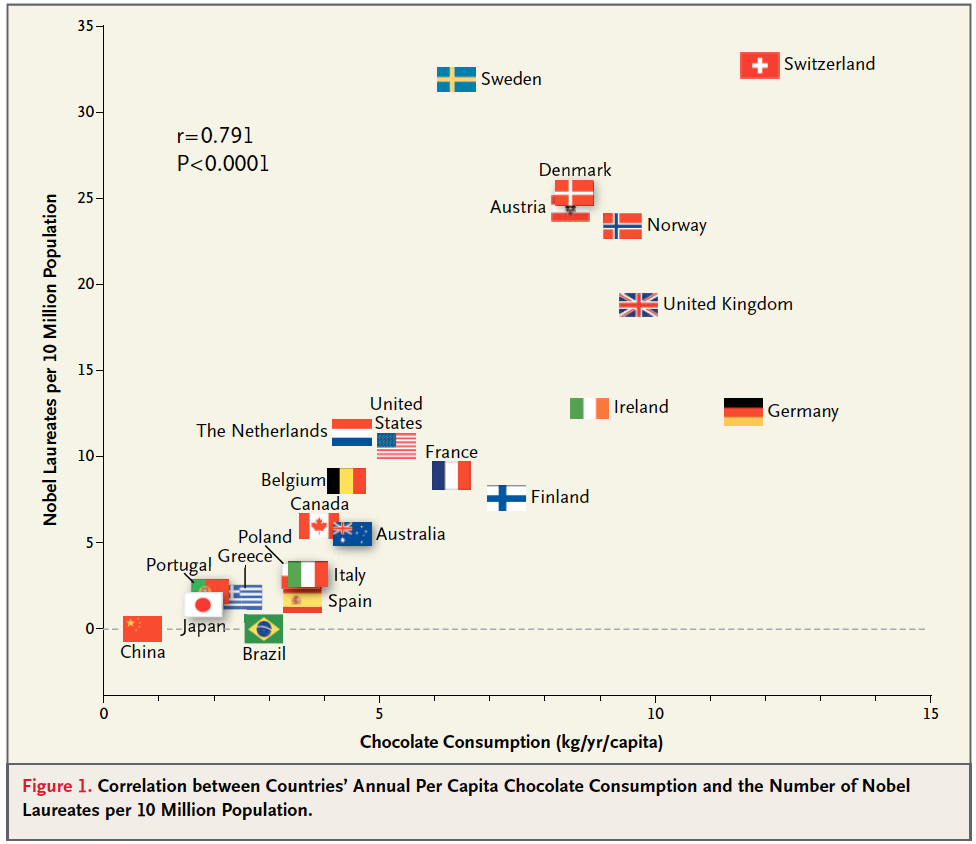
\includegraphics[width=0.8\textwidth]{chocolate_nobel.png}
\end{frame}

\begin{frame}{Hypothesis 1: $N$ causes $C$}
  ``Nobel prizes are celebrated with massive chocolate feasts''\\

  $\Sin = \{N\}$, $\Send = \{C\}$, $\Srnd = \emptyset$, $\theta = (\alpha,\beta) \in \RN^2$, $\C{X}_N = \RN$, $\C{X}_C = \RN$, $f_{\alpha,\beta} : (x_N,x_C) \mapsto \alpha + \beta x_N$.

  Structural equations:
    $$X_C^{\doit(x_N)} = \alpha + \beta x_N.$$
  
  For a given parameter $(\alpha,\beta)$, the SCM has a unique solution function 
  $$g_{\alpha,\beta} : x_N \mapsto \alpha + \beta x_N,$$
  unique potential outcomes of the form 
  $$X_C^{\doit(x_N)} = \alpha + \beta x_N,$$
  and any conditional random variable $X : \C{U} \times \CXJ \to \CX$ that satisfies
  $$X_C = \alpha + \beta X_N$$
  is a solution of $M$.
\end{frame}

\begin{frame}{Hypothesis 2: $W$ causes $N$ and $C$}
  ``Inhabitants of wealthy countries can eat more chocolate and conduct more scientific research''\\

  $\Sin = \emptyset$, $\Send = \{C,N\}$, $\Srnd = \{W\}$, $\theta = (\alpha,\beta,\gamma,\delta,\sigma) \in \RN^4 \times [0,\infty)$, $\C{X}_W = \RN$, $\C{X}_C = \RN$, $\C{X}_N = \RN$, $f_{\theta} : (x_C,x_N,x_W) \mapsto (\alpha + \beta x_W, \gamma + \delta x_W) \in \C{X}_C \times \C{X}_N$, $P_{\theta} = \C{N}(0,\sigma^2)$.

  Structural equations:
    \begin{align*}
      X_C & = \alpha + \beta X_W, \\
      X_N & = \gamma + \delta X_W.
    \end{align*}
  
  For a given parameter $\theta$, the SCM $M_{\theta}$ has unique solution function 
  $$g_\theta : x_W \mapsto (\alpha + \beta x_W, \gamma + \delta x_W) \in \C{X}_C \times \C{X}_N$$
  and potential outcomes of the form
  $$(X_C,X_N) = (\alpha + \beta X_W, \gamma + \delta X_W)$$ 
  for any random variable $X_W \sim \C{N}(0,\sigma^2)$.
\end{frame}

\begin{frame}{Hard interventions}
  \begin{Def}
  Let $M = \lt \Sin, \Send, \Srnd, \CX, P, f \rt$ be an SCM and
  $T \subseteq J \cup V \cup W$ the \emph{intervention target}. We define three variants of \emph{hard interventions}:
    \begin{enumerate}
      \item For a \emph{specified target value} $\xi_T \in \CX_T$, define
    $$M_{\doit(X_T=\xi_t)} = \lt J\setminus T, V \cup T, W \setminus T, \CX, P_{W\setminus T}, (f_{V\setminus T},\xi_T)\rt$$
  \item For a \emph{stochastic target value} with distribution $Q_T \in \bigotimes_{t\in T} \C{P}(\CX_t)$, define
    $$M_{\doit(X_T\sim Q_T)} = \lt J\setminus T, V \setminus T, W \cup T, \CX, P_{W\setminus T} \otimes Q_T, f_{V\setminus T}\rt$$
  \item For an \emph{unspecified target value}, define
    $$M_{\doit(T)} = \lt J\cup T, V\setminus T, W \setminus T, \CX, P_{W\setminus T}, f_{V\setminus T} \rt$$
    \end{enumerate}
  \end{Def}
\end{frame}

\begin{frame}{Hard interventions commute}
%In the following slides, we always consider an SCM
%$\C{M} = \langle \Sin, \Send, \Srnd, \CX, P, f \rangle$.

\begin{block}{Proposition}
Hard interventions $\doit(T_1\dots)$, $\doit(T_2\dots)$ with disjoint targets $T_1, T_2 \subseteq \Sin \cup \Srnd \cup \Send$ (of any of the three variants) commute:
  $$(\C{M}_{\doit(T_1\dots)})_{\doit(T_2\dots)} = (\C{M}_{\doit(T_2\dots)})_{\doit(T_1\dots)}.$$
\end{block}
Try proving this yourself!
\end{frame}

\begin{frame}{Soft interventions}
%Soft interventions replace the causal mechanism of an endogenous variable by another causal mechanism,
%or the exogenous distribution of an exogenous random variable by another distribution.
\begin{Def}
  Given an SCM $M = \lt \Sin, \Send, \Srnd, \CX, P, f \rt$
  and an intervention target $T \subseteq \Send \cup \Srnd$, a \emph{soft intervention on $M$ targeting $T$}
  yields an intervened SCM of the form
  $$\tilde{M} := \lt \Sin,\Send,\Srnd,\CX,\tilde{P},\tilde{f} \rt$$
  where
  $$\tilde{P} = \lp\bigotimes_{w \in \Srnd \sm T} P_w \rp \otimes \lp \bigotimes_{w \in T \cap \Srnd} \tilde{P}_w \rp$$
  and
  $$\tilde{f}(x) = \begin{cases}
      f_v(x) & v \in \Send\sm T \\
      \tilde{f}_v(x) & v \in T \cap \Send \\
  \end{cases}$$
  for some distributions $\tilde{P}_w \in \C{P}(\CX_w)$ and measurable functions $\tilde{f}_v : \CX \to \CX_v$.
\end{Def}
\end{frame}

\begin{frame}{Intervention variables---Example}
  \emph{Intervention variables} encode whether/how an intervention is performed.
  \begin{example}
    Consider an SCM with endogenous variables $X_1,X_2$, exogenous random variables $E_1,E_2$ and structural equations:
    $$X_1 = f_1(X_2,E_1), \qquad
      X_2 = f_2(X_1,E_2) \phantom{x_2}$$
    After a hard intervention $\doit(X_2=x_2)$ the structural equations become:
    $$X_1 = f_1(X_2,E_1), \qquad
      X_2 = x_2 \phantom{f_2(X_1,E_2)}$$
    We can combine both into a single SCM by adding an intervention variable $I_2$ (an exogenous input variable) and change the structural equations into:
    $$X_1 = f_1(X_2,E_1), \qquad
      X_2 = \begin{cases}
        f_2(X_1,E_2) & I_2 = 0 \\
        x_2          & I_2 = 1
      \end{cases}$$
  \end{example}
\end{frame}

\begin{frame}{Intervention variables---Remarks}
  \begin{itemize}
     \item Intervention variables encode whether/how an intervention is performed.
     \item No rigorous definition; the question of how to use intervention variables is a modeling issue.
     \item Examples: 
       \begin{itemize}
         \item coin flip in RCT that decides treatment/control group (binary);
         \item dose of treatment with a drug (continuous).
       \end{itemize}
     \item Can be modeled as exogenous input variables, exogenous random variables, or endogenous variables.
  \end{itemize}       
\end{frame}

\begin{frame}{Decomposition}

If we think about an SCM as modeling a ``system'', then we also obtain a model for any ``subsystem'' in the following way.
\begin{Def}[Taking a submodel of an SCM]\label{def:sub_scm}
  Given an SCM $M = \lt \Sin, \Send, \Srnd, \CX, P, f \rt$, subsets $V' \subseteq V$ and $W' \subseteq W$, we define its \emph{submodel on $V' \dcup W'$} as the SCM
  $$\lt \Sin \cup (V \sm V') \cup (W \sm W'), V', W',\CX,P_{W'},f_{V'} \rt.$$
\end{Def}
  Note that this is just the intervened SCM $M_{\doit((V\cup W) \sm (V' \cup W'))}$.
\end{frame}

\begin{frame}{Composition}
%Given two SCMs, such that some of the variables of one SCM can be used as (part of the) exogenous input of the other, and possibly vice versa, we can compose them into a single SCM.
\begin{Def}[Composing two SCMs]\label{def:compose_scm}
  Given two SCMs $M_1 = \lt \Sin_1, \Send_1, \Srnd_1, \CX_1, P_1, f_1 \rt$ and $M_2 = \lt \Sin_2, \Send_2, \Srnd_2, \CX_2, P_2, f_2 \rt$ and two subsets $C_1 \subseteq \Sin_1 \cap (\Send_2 \cup \Srnd_2)$ and $C_2 \subseteq (\Send_1 \cup \Srnd_1) \cap \Sin_2$ satisfying the following conditions:
  (i) for all $c \in C_1 \cup C_2$: $(\CX_1)_c = (\CX_2)_c$,
  (ii) $(\Sin_1 \sm C_1) \cap (\Sin_2 \sm C_2) = \emptyset$,
  (iii) $\Send_1 \cap \Send_2 = \emptyset$,
  (iv) $\Srnd_1 \cap \Srnd_2 = \emptyset$,

  we define the \emph{composed SCM}
  $$M_{12} := \lt (\Sin_1 \sm C_1) \dcup (\Sin_2 \sm C_2), \Send_1 \dcup \Send_2, \Srnd_1 \dcup \Srnd_2, \CX_{12}, P_{12} \rt,$$
  where
  \begin{align*}
    \CX_{12} &:= (\CX_1)_{(\Sin_1 \sm C_1) \dcup \Send_1 \dcup \Srnd_1} \times (\CX_2)_{(\Sin_2 \sm C_2) \dcup \Send_2 \dcup \Srnd_2}, \\
    P_{12} &:= P_1 \otimes P_2, \\
    f_{12} &:= (f_1, f_2).
  \end{align*}
\end{Def}
\end{frame}

\begin{frame}{Modularity}
  \begin{itemize}
    \item Decomposition (taking submodels) is `dual to' composition (combining submodels).
    \item These operations formalize the notion of \emph{modularity}: an SCM models a system of interacting components.
    \item The submodels on individual variables correspond with `atomic' subsystems that cannot be decomposed into smaller parts.
  \end{itemize}
\end{frame}

\begin{frame}{Unique solvability}
\begin{definition}
  $M$ is called \emph{uniquely solvable} if it has a unique solution function. 
\end{definition}
%\begin{example}
%  An SCM with endogenous real variables $X,Y$, and exogenous real random variable $E$, and structural equations
%  $$X = Y, \qquad Y = X$$
%  is not uniquely solvable.
%
%  If it had structural equations
%  $$X = E, \qquad Y = X$$
%  instead, it would be 
%  uniquely solvable.
%\end{example}
\end{frame}

\begin{frame}{Unique solvability properties}
\begin{theorem}
  \begin{enumerate}
    \item $M$ is uniquely solvable if and only if 
      for all $\xW\in\CXW$, for all $\xJ \in \CXJ$, the equation
      $$\xV = f(\xV,\xJ,\xW)$$
      has a unique solution for $\xV\in\CXV$.
%    \item If $M$ is uniquely solvable, then for all $\xJ\in\CXJ$, $M_{\doit(\XJ=\xJ)}$ is uniquely solvable.
    \item If $M$ is uniquely solvable, it has a unique Markov kernel
      $$P_{M}(X_V,X_W \mid \doit(X_J)) := (g,\id_{\CXW})_* \lp \bigg( \bigotimes_{w\in\Srnd} P_w(X_w) \bigg) \otimes \delta(X_J|X_J) \rp$$
      where $g$ is the solution function of $M$.
  \end{enumerate}
\end{theorem}
\begin{definition}
  If a subset of variables $O \subseteq V \cup W$ is considered observed, its marginal
  $P_{M}(X_O \mid \doit(X_J))$ is called the \emph{observational Markov kernel of $M$}.
\end{definition}
\end{frame}

%\begin{frame}{Proof ideas}
%  \begin{enumerate}
%    \item Apart from checking the definitions, we have to prove that the solution function is measurable.
%This follows (with some more advanced measure theory) from the measurability of the causal mechanism $f$.
%
%    \item Let $g : \CXJ \times \CXW \to \CXV$ be the unique solution function of $M$.
%      The Markov kernel is obtained as the push-forward
%      $$P_{M}(\XV,\XW \mid \XJ) = (g,\id_{\CXW})_* P(\XW \mid \XJ)$$
%      of the exogenous distribution of $M$, interpreted as a constant Markov kernel $\CXJ \dshto \CXW$:
%  $$P(\XW \mid \XJ) := \bigotimes_{k\in\Srnd} P(X_k).$$
%  Equivalently, for all $\xJ \in \XJ$,
%      $$P_{M}(\XV,\XW \mid \XJ=\xJ) = P((g(\xJ,\XW),\XW))$$
%      for a random variable $\XW \sim P$. The uniqueness of $P_{M}$ follows eventually from the uniqueness of $g$.
%  \end{enumerate}
%\end{frame}

\begin{frame}{Example: Linear SCMs}
  \begin{Def}
We call an SCM $M=\lt \Sin, \Send, \Srnd, \CX, P, f \rt$
\emph{linear} if all variables are real-valued and
each component of the causal mechanism is an affine combination of endogenous variables, that is
$$
%  f_v(x) = \sum_{w\in V \cup J \cup W} B_{vw} x_w,
    f_v(x) = \sum_{u\in V} B_{vu}(x_J,x_W) x_u + c_v(x_J,x_W),
$$
    where $B(x_J,x_W)\in\RN^{V \times V}$ is a matrix-valued function $\CXJ\times\CXW \to \RN^{V\times V}$ and
$c(x_J,x_W) \in \RN^V$ is a vector-valued function $\CXJ\times\CXW \to \RN^V$.
  \end{Def}

  \begin{Prp}
Let $L \subseteq V$.
$(M)_{\doit(V\setminus L)}$ is uniquely solvable if and only if 
$I_{L}-B_{LL}(x_J,x_W)$ are invertible $\forall x_J \in \CX_J, x_W \in \CX_W$,
with unique solution function:
\small
  \begin{equation*}\begin{split}
    g &: \RN^{V\setminus L} \times \RN^{J\cup W} \to \RN^L \\
      &: (x_{V\setminus L},x_J,x_W) \mapsto (I_L - B_{LL}(x_J,x_W))^{-1} \big(B_{L,{V\setminus L}}(x_J,x_W) x_{V\setminus L} + c_{L}(x_J,x_W)\big).
  \end{split}\end{equation*}
  \end{Prp}
\end{frame}

\begin{frame}{Simple SCMs}
For simplicity, we consider mostly ``simple SCMs'':
\begin{definition}
  An SCM $M$ is called \emph{simple} if the intervened SCM
  $M_{\doit(T)}$ is uniquely solvable for all $T \subseteq \Sin \cup \Send \cup \Srnd$. 
\end{definition}
Note that this includes unique solvability of $M$ itself for $T = \emptyset$.
\begin{corollary}
  If $M$ is simple, and $O \subseteq V \cup W$ is considered observed, then the
  observational Markov kernel $P_{M}(X_O \mid \doit(X_J))$
  and all its \emph{interventional Markov kernels}
  $$P_{M}(X_{O\setminus T} \mid \doit(X_J),\doit(X_T)) := P_{M_{\doit(T)}}(X_{O\setminus T} \mid \doit(X_{J \cup T}))$$
  for $T \subseteq O$ exist and are unique.
\end{corollary}
\end{frame}

\begin{frame}{Example of simple SCM}
\begin{example}
Consider an SCM with structural equations
$$X_1 = W_1 \qquad X_2 = W_2 \qquad X_3 = X_1 X_4 + W_3 \qquad X_4 = X_2 X_3 + W_4 $$
where the $X$'s are considered endogenous real variables and the $W$'s exogenous variables with domains $(-1,1)$.
We can solve the system of structural equations with respect to $X$ in terms of $W$:
$$X_1 = W_1 \qquad X_2 = W_2 \qquad X_3 = \frac{W_3 + W_1 W_4}{1 - W_1 W_2} \qquad X_4 = \frac{W_2 W_3 + W_4}{1 - W_2 W_1}$$
Similarly, we can take any subset of the structural equations and solve it with respect to the variables appearing on the l.h.s.\ in terms of the variables appearing on the r.h.s.\ of the equations in the subset, and obtain a unique solution. Thus this SCM is simple.
%For example, only solving the structural equations for $X_3$ and $X_4$, we obtain:
%$$X_3 = \frac{W_3 + W_1 W_4}{1 - W_1 X_2} \qquad X_4 = \frac{W_2 W_3 + W_4}{1 - W_2 X_1}$$
%where the variables $X_1$ and $X_2$ are now considered as exogenous input variables (instead of endogenous variables).
%Hence, any subset of the structural equations has a unique solution for the variables appearing on the l.h.s.\ in terms
%of the remaining ones on the r.h.s., which means that this SCM is simple.
\end{example}
We will see later that all acyclic SCMs are simple.
\end{frame}

\begin{frame}{Relations between causal models}
  \centerline{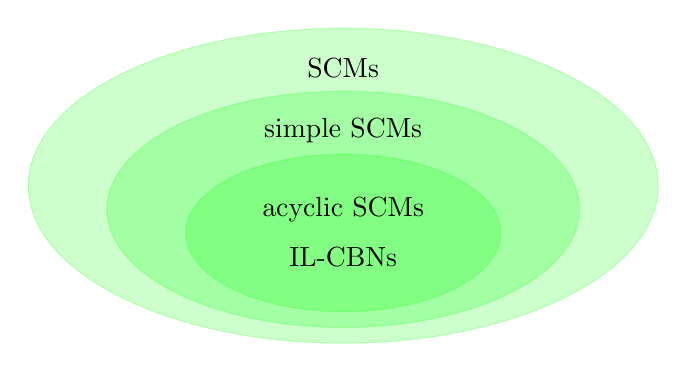
\begin{tikzpicture}
      \begin{scope}
%        \draw[draw=green,fill=green,opacity=0.2] (0,0) ellipse (1.5cm and 0.5cm);
        \draw[draw=green,fill=green,opacity=0.2] (0,0.3) ellipse (2cm and 1cm);
        \draw[draw=green,fill=green,opacity=0.2] (0,0.6) ellipse (3cm and 1.5cm);
        \draw[draw=green,fill=green,opacity=0.2] (0,0.9) ellipse (4cm and 2cm);
        \node at (0,0) {IL-CBNs};
        \node at (0,0.6) {acyclic SCMs};
        \node at (0,1.6) {simple SCMs};
        \node at (0,2.4) {SCMs};
      \end{scope}
  \end{tikzpicture}}

  \bigskip
  IL-CBNs are equivalent to acyclic SCMs.
  Simple SCMs are more expressive than IL-CBNs, because they can model causal cycles (e.g., feedback loops) to some extent.
  The class of SCMs can deal with more severe forms of feedback at the cost of much complexity.
\end{frame}

